% Data flow diagram
% Author: David Fokkema
\documentclass{article}
\usepackage{tikz}
\usetikzlibrary{shapes,arrows}
\usepackage{pdflscape}
\usepackage[papersize={6.5cm, 6.6cm}, text={6.5cm, 6.6cm}]{geometry}
\usetikzlibrary{decorations.text}
\usepackage{xcolor}
% \selectcolormodel{gray}

\begin{document}
\thispagestyle{empty}
%\begin{landscape}
\begin{center}
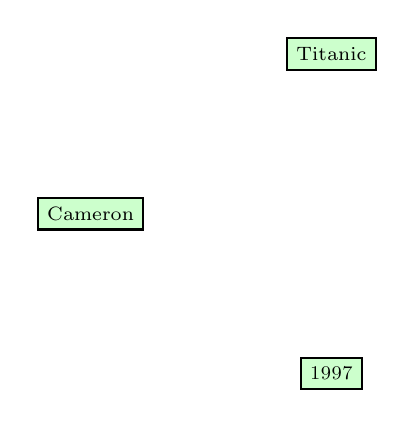
\begin{tikzpicture}[
  font=\sffamily,
  every matrix/.style={ampersand replacement=\&,column sep=0.9cm,row
sep=0.8cm,font=\scriptsize},
  entity/.style={draw,thick,rectangle,fill=green!20},
  word/.style={draw,thick,ellipse,fill=blue!20,},
  mediator/.style={draw,thick,circle},
  entityType/.style={draw,thick,rounded corners,fill=yellow!20,inner
sep=.3cm},
  mathType/.style={draw,thick,diamond,fill=red!20},
  mediatorToEntity/.style={->,>=stealth',shorten
>=1pt,semithick,black,sloped,above,font=\sffamily\scriptsize},
  typeToEntity/.style={->,>=stealth',shorten
>=1pt,semithick,black,sloped,above,font=\sffamily\scriptsize},
  wordToEntity/.style={-,>=stealth',shorten >=1pt,ultra
thick,dotted,blue,sloped,above,font=\sffamily\scriptsize},
  entityToMath/.style={->,>=stealth',shorten >=1pt,ultra
thick,dashed,violet,sloped,above,font=\sffamily\scriptsize},
  every node/.style={align=center}]

  % Cameron directed Titanic in 1997.
  
  % Position the nodes using a matrix layout
  \matrix{ 
    \&  \& \node[entity] (eTitanic)
{Titanic}; \\
      \&  \& 
\\
    \node[entity] (eCameron) {Cameron}; \&  \& \\
     \&  \&  \\
     \& \& \node[entity][font=\sc\scriptsize] (e1997) {1997}; \\
  };
 
  % words to entities
  % \draw [wordToEntity] (wCameron) edge node {}  (eCameron);
  % \draw [wordToEntity] (wTitanic) edge node {}  (eTitanic);
  % \draw [wordToEntity] (w1997) edge node {}  (e1997);
  
  % event word to mediators
  % \draw [wordToEntity] (wDirected) edge node {}  (m1);
  % \draw [wordToEntity] (wDirected) edge node {}  (m2);
  % \draw [wordToEntity] (wDirected) edge node {}  (m3);
  
  % mediator to entities
  % \draw [mediatorToEntity] (m1) edge node {directed\\.arg1}  (eCameron);
  % \draw [mediatorToEntity] (m1) edge node
% {\hspace{-0.5cm}directed\\\hspace{-0.5cm}.arg2} 
%(eTitanic);
  
 % \draw [mediatorToEntity] (m2) edge node {directed.in}  (e1997);
  % \draw [mediatorToEntity] (m2) edge node[rotate=180] {directed.arg2} 
%(eTitanic);
  
 % \draw [mediatorToEntity] (m3) edge node[below] {directed.arg1} 
% (eCameron);
  % \draw [mediatorToEntity] (m3) edge node[below] {directed.in}  (e1997);
  
  
  
\end{tikzpicture}
\end{center}
\end{document}
